\documentclass[tikz,border=1.25mm]{standalone}
\usetikzlibrary{matrix, positioning, shapes, fit, shapes.geometric, backgrounds, arrows.meta}
\usepackage{amssymb}

\definecolor{kellygreen}{rgb}{0.3, 0.73, 0.09}
\definecolor{darkgray}{rgb}{0.30, 0.30, 0.30}
\definecolor{gray}{rgb}{0.53, 0.53, 0.53}
\definecolor{slate}{rgb}{0.094,0.094,0.094}
\definecolor{cobalt}{rgb}{0.244,0.364,0.972}

\begin{document}

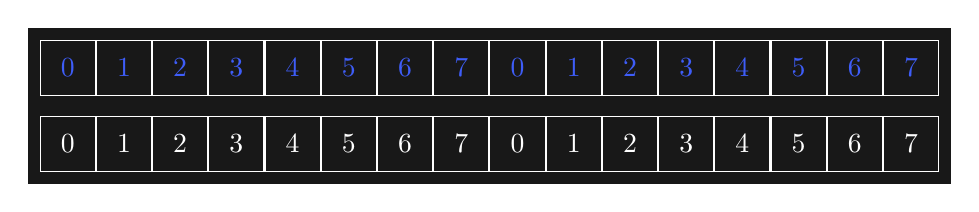
\begin{tikzpicture}[
  background rectangle/.style={fill=slate},
  show background rectangle,
  every node/.style={
    color=white,
    text=white,
    draw,
    inner sep=0mm,
    minimum height=7mm,
    minimum width=7mm
  },
]

\matrix(m)[
  matrix anchor=north west,
  matrix of nodes,
  nodes in empty cells,
  column sep=0mm,
  row sep=2.5mm,
  every odd row/.style={nodes={text=cobalt}},
  draw=none
] {
  0 & 1 & 2 & 3 & 4 & 5 & 6 & 7 & 0 & 1 & 2 & 3 & 4 & 5 & 6 & 7 \\
  0 & 1 & 2 & 3 & 4 & 5 & 6 & 7 & 0 & 1 & 2 & 3 & 4 & 5 & 6 & 7 \\
};

\end{tikzpicture}

\end{document}
